% Informe E3 en formato IEEE (clase IEEEtran, modo conference; TeX Live texlive-publishers). Compilar: pdflatex x2.
\documentclass[conference]{IEEEtran}
\usepackage[utf8]{inputenc}\usepackage[T1]{fontenc}\usepackage{booktabs,array,hyperref,microtype,graphicx}
\hypersetup{colorlinks=true,linkcolor=black,urlcolor=blue}
\title{Puntos autom\'aticos DINOv3 para SAM~2.1 en la segmentaci\'on de agua superficial en Sentinel-2 (Sen1Floods11): informe E3}
\author{\IEEEauthorblockN{E.~Villarreal and R.~Ch\'avez}
\IEEEauthorblockA{PUCP, Ingenier\'ia Inform\'atica, Deep Learning 1INF52 (2026-2)\\
Repositorio: github.com/roberto-chavez/auto-prompt-sam2\\
\textit{Retroalimentaci\'on del workshop (18--20 nov): pendiente de confirmaci\'on}}}
\begin{document}\maketitle
\begin{abstract}
Estudiamos cu\'anto cambia la calidad de SAM~2.1 al sustituir puntos simulados desde etiquetas por puntos autom\'aticos derivados de DINOv3 para segmentar agua superficial (incluida agua permanente) en Sentinel-2. Con presupuesto nominal igualado (3+/3$-$ por componente) y decoder congelado, el IoU de agua en validaci\'on pasa de 0.154 (referencia asistida) a 0.299 (\emph{official}) y de 0.152 a 0.317 (\emph{leave\_paraguay\_out}); la hip\'otesis previa de que los puntos autom\'aticos quedar\'ian por debajo de la referencia asistida queda refutada en validaci\'on. Los totales reales de puntos de ambos brazos no se han verificado. Entrenar solo el mask decoder eleva el IoU a 0.484/0.506, un factor distinto del tipo de prompt. Ning\'un conjunto reservado se ha abierto: no hay evidencia de transferencia geogr\'afica.
\end{abstract}

\section{Problema y pregunta}
SAM~2.1 \cite{ravi2024sam2} segmenta a partir de prompts, pero las im\'agenes satelitales carecen de un usuario que los coloque. La pregunta del proyecto es: \emph{¿cu\'anto cambia la calidad al sustituir puntos simulados desde etiquetas por puntos autom\'aticos derivados de DINOv3 \cite{simeoni2025dinov3}?} La tarea es segmentar \textbf{agua superficial}, incluida el agua permanente; no se afirma detectar solo inundaciones recientes.

\section{Datos, particiones y preprocesamiento}
Usamos Sen1Floods11 \cite{bonafilia2020sen1floods11} (chips Sentinel-2 con etiqueta manual). Dos reg\'imenes: \emph{official} (252 train / 89 val) y \emph{leave\_paraguay\_out} (213/75), con Bolivia y Paraguay reservados sin abrir. Las configuraciones se fijan con train/val; los reservados no se han tocado. El flujo autom\'atico consume solo imagen, caracter\'isticas y validez; la sonda de agua se entrena con etiquetas de train (no es un sistema libre de etiquetas). M\'etrica principal: IoU de agua acumulado (pooled); precisi\'on, recall y Dice la explican.

\subsection{Protocolo y comparabilidad (antecedente)}
\begin{table}[!t]\centering\footnotesize\caption{Diferencias que afectan la interpretaci\'on de cada fila.}
\begin{tabular}{@{}p{1.7cm}p{2.0cm}p{1.9cm}p{1.5cm}@{}}\toprule
Fila & Origen de componentes & Puntos & Decoder\\\midrule
Etapa 3 & etiqueta (real) & 1+/1$-$ & congelado\\
Etapa 5 & predicci\'on DINOv3 & $\le$3+/3$-$ & congelado\\
Malla & SAM 32$\times$32 + DINOv3 & autom\'atico & congelado\\
Etapa 6 & predicci\'on DINOv3 & $\le$3+/3$-$ & entrenado\\\bottomrule
\end{tabular}\end{table}
El evaluador (IoU acumulado sobre p\'ixeles v\'alidos), el preprocesamiento y las particiones son los mismos en todas las filas; lo que cambia es la columna anterior. Por eso etapa~3 vs.\ etapa~5 mezcla dos factores (origen de componentes y presupuesto) y etapa~5 vs.\ etapa~6 cambia el decoder. Cada factor debe aislarse con la matriz de la etapa~7 (A1: fuente de prompt con presupuesto 3+/3$-$ igualado; A2: barridos de $k$; A3: congelado vs.\ ajustado con la misma ruta).

\begin{table}[!t]\centering\footnotesize\caption{Tama\~no de las particiones y objetivos de la sonda (etapa 5).}
\begin{tabular}{@{}lrrrr@{}}\toprule
R\'egimen & train & val & p\'x agua (train) & p\'x no agua\\\midrule
official & 252 & 89 & 19\,538 & 192\,017\\
leave\_paraguay\_out & 213 & 75 & 16\,660 & 158\,771\\\bottomrule
\end{tabular}\end{table}
Los p\'ixeles de la tabla son celdas de la rejilla de caracter\'isticas $32{\times}32$; 46\,493 (official) y 42\,681 (excluido) celdas se ignoran por validez. Cada r\'egimen tiene su propio escalador y sonda, de modo que ninguna estad\'istica de validaci\'on ni de Paraguay reservado entra en el ajuste.

\section{L\'inea base y teardown}
Modelo \texttt{facebook/sam2.1-hiera-tiny} (Apache-2.0): 38\,962\,498 par\'ametros (encoder de imagen 27.2\,M; mask decoder 4\,215\,109; encoder de prompts 6\,220; memoria y proyecciones 7.5\,M) y 296.05~GFLOPs contados (parcial). Con 1+/1$-$ puntos tomados de etiquetas y decoder congelado, el IoU en validaci\'on es 0.158 (official): recall alto (0.894) y precisi\'on baja (0.161), es decir, sobre-segmentaci\'on.

\begin{table}[!t]\centering\footnotesize\caption{Teardown de SAM~2.1 hiera-tiny (conteos reproducibles con \texttt{scripts/teardown\_architecture\_counts.py}).}
\begin{tabular}{@{}lr@{}}\toprule
Bloque & Par\'ametros\\\midrule
Encoder de imagen (Hiera) & 27\,219\,136\\
Mask decoder & 4\,215\,109\\
Memoria y proyecciones & 7\,520\,736\\
Encoder de prompts & 6\,220\\
Residual & 1\,297\\\midrule
Total & 38\,962\,498\\\bottomrule
\end{tabular}\end{table}
El mask decoder es solo el 10.8\,\% de los par\'ametros (4\,215\,109 de 38\,962\,498); por eso es el candidato econ\'omico para adaptar sin tocar el encoder, que concentra el 69.9\,\%. El m\'odulo de memoria no interviene en la inferencia sobre una imagen.

\section{M\'etodo autom\'atico e intervenci\'on del decoder}
\textbf{Puntos.} Caracter\'isticas DINOv3 ViT-L/16 SAT-493M congeladas (32$\times$32$\times$1024) $\to$ sonda log\'istica supervisada $\to$ mapa de probabilidad $\to$ componentes y hasta 3+/3$-$ puntos por componente $\to$ SAM (m\'ascara de mayor IoU predicho) $\to$ uni\'on. Se compar\'o tambi\'en una malla de SAM puntuada con DINOv3. La configuraci\'on elegida (C=0.1, umbral 0.7) deja 28/89 y 24/75 chips sin componentes (m\'ascara vac\'ia).\\
\textbf{Decoder.} Se entrena solo el mask decoder (4\,215\,109 par\'ametros; BCE+Dice sobre p\'ixeles v\'alidos; AdamW $10^{-5}$, 10 \'epocas, FP32), con encoder de imagen y de prompts congelados.

\section{Resultados (solo validaci\'on)}
\begin{table}[!t]\centering\footnotesize\caption{IoU de agua en validaci\'on (cifras recalculadas desde las salidas originales con \texttt{scripts/e3\_collect\_results.py}).}
\begin{tabular}{@{}p{3.6cm}rrrr@{}}\toprule
Fila & IoU & Prec. & Rec. & Dice\\\midrule
\multicolumn{5}{@{}l}{\emph{official} (89 chips)}\\
Etiq. 1+/1$-$, congelado & .158 & .161 & .894 & .273\\
DINOv3 $\le$3+/3$-$, congelado & .299 & .327 & .774 & .460\\
Malla SAM+DINOv3, congelado & .179 & .922 & .181 & .303\\
DINOv3, decoder entrenado (\'ep.~10) & .484 & .688 & .620 & .652\\\midrule
\multicolumn{5}{@{}l}{\emph{leave\_paraguay\_out} (75 chips)}\\
Etiq. 1+/1$-$, congelado & .168 & .169 & .969 & .288\\
DINOv3 $\le$3+/3$-$, congelado & .317 & .354 & .750 & .481\\
Malla SAM+DINOv3, congelado & .209 & .906 & .213 & .345\\
DINOv3, decoder entrenado (\'ep.~8) & .506 & .738 & .617 & .672\\\bottomrule
\end{tabular}\end{table}
\begin{figure}[!t]\centering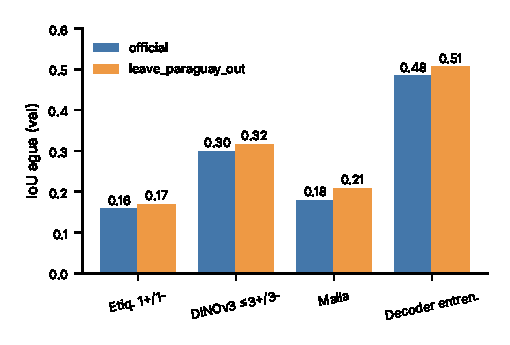
\includegraphics[width=\columnwidth]{fig_iou.pdf}\caption{IoU de agua en validaci\'on por fila (mismos datos que la tabla de resultados). Las filas no son todas comparables entre s\'i (ver texto).}\end{figure}
\textbf{Puntos simulados vs.\ autom\'aticos (decoder congelado).} Antecedente descriptivo (etapas 3 y 5): los puntos autom\'aticos duplican el IoU en ambos reg\'imenes, a costa de menos recall y m\'as precisi\'on. \emph{Salvedad que afecta la interpretaci\'on:} los puntos de etiqueta son 1+/1$-$ por componente real, los autom\'aticos hasta 3+/3$-$ por componente predicho (presupuestos reales 1\,204+/2\,055$-$ en official). No es una comparaci\'on con presupuesto igualado. La comparaci\'on con referencia asistida igualada se ejecut\'o despu\'es, en la etapa~7 (secci\'on siguiente).\\
\begin{figure}[!t]\centering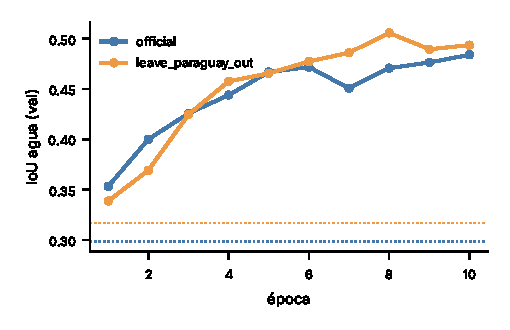
\includegraphics[width=\columnwidth]{fig_curvas.pdf}\caption{IoU de validaci\'on por \'epoca del decoder entrenado (etapa 6); las l\'ineas punteadas son la etapa 5 congelada.}\end{figure}
\begin{table}[!t]\centering\footnotesize\caption{Etapa 6: m\'etricas de validaci\'on por \'epoca (de \texttt{curves.json}).}
\begin{tabular}{@{}rrrrr@{}}\toprule
\'Ep. & IoU off. & Dice off. & IoU excl. & Dice excl.\\\midrule
1 & 0.353 & 0.522 & 0.339 & 0.506\\
2 & 0.400 & 0.572 & 0.369 & 0.539\\
3 & 0.426 & 0.597 & 0.425 & 0.596\\
4 & 0.444 & 0.615 & 0.458 & 0.628\\
5 & 0.467 & 0.637 & 0.466 & 0.635\\
6 & 0.472 & 0.641 & 0.477 & 0.646\\
7 & 0.451 & 0.621 & 0.486 & 0.654\\
8 & 0.471 & 0.640 & 0.506 & 0.672\\
9 & 0.476 & 0.645 & 0.490 & 0.657\\
10 & 0.484 & 0.652 & 0.494 & 0.661\\
\bottomrule\end{tabular}\end{table}
\textbf{Congelado vs.\ ajustado.} Ajustar el decoder suma +18.5 pp (official) y +18.9 pp (excluido) respecto a la etapa 5, con una semilla; la mejor \'epoca y el umbral se eligieron en la misma validaci\'on. Es un efecto del decoder, no del prompt. En la intervenci\'on preliminar E2 (40 chips, puntos simulados, semilla 42) el IoU pas\'o de 0.170 a 0.308 en la \'epoca 1 y cay\'o a 0.150 en la \'epoca 4: el ajuste es inestable.\\
\textbf{Transferencia.} \emph{No evaluada.} La diferencia entre reg\'imenes ocurre en poblaciones de validaci\'on distintas y no prueba transferencia geogr\'afica.

\section{Intervenci\'on E2 previa}
\begin{table}[!t]\centering\footnotesize\caption{E2: 40 chips de validaci\'on, puntos simulados, semilla 42, official.}
\begin{tabular}{@{}lrrrr@{}}\toprule
Brazo & IoU & Prec. & Rec. & Dice\\\midrule
Congelado & .170 & .171 & .964 & .291\\
Ajustado, mejor \'ep.~1 & .308 & .399 & .575 & .471\\\bottomrule
\end{tabular}\end{table}
La mejora de la mejor \'epoca proviene de menos falsos positivos (precisi\'on $.171\to.399$) a costa de recall ($.964\to.575$); la \'ultima \'epoca (IoU .150) muestra que el criterio de parada importa. Este resultado usa un subconjunto de 40 chips y no es comparable de forma directa con las 89 im\'agenes de las etapas 5--6.

\section{Etapa 7 ejecutada: ablaciones A1--A3}
La etapa~7 se ejecut\'o en Colab (notebook 07 ejecutado, commit \texttt{ebde34e}) sobre las 13 filas y las validaciones de ambos reg\'imenes (89 y 75 chips), sin entrenar ni recalibrar (se reutilizan sonda, umbrales y mejor \'epoca de las etapas 5--6) y sin abrir conjuntos reservados. Los valores de control coinciden con la salida del notebook: official 0.1540 / 0.2986 / 0.4841 y excluido 0.1515 / 0.3168 / 0.5058 (asistido igualado / autom\'atico / decoder ajustado). Adem\'as, la etapa~7 reproduce \emph{exactamente} las cifras de las etapas 3 y 5 (fila hist\'orica 0.1580/0.1684; puntos 0.2986/0.3168; malla 0.1785/0.2088), lo que respalda la consistencia de la re-ejecuci\'on.
\begin{table}[!t]\centering\scriptsize\caption{A1 (etapa 7, decoder congelado, val.): IoU de agua (prec., recall).}
\begin{tabular}{@{}p{2.6cm}p{2.5cm}p{2.5cm}@{}}\toprule
Fila & official (89) & excluido (75)\\\midrule
DINOv3 $\le$3+/3$-$ (auto) & .299 (.327, .774) & .317 (.354, .750)\\
Etiq. 3+/3$-$ (asistida igualada) & .154 (.155, .960) & .152 (.152, .974)\\
Etiq. 1+/1$-$ (hist\'orica) & .158 (.161, .894) & .168 (.169, .969)\\
Malla SAM+DINOv3 & .179 (.922, .181) & .209 (.906, .213)\\
Caja completa (control) & .098 (.099, .872) & .100 (.102, .887)\\
\bottomrule\end{tabular}\end{table}
\textbf{A1: qu\'e cambia.} Solo la fuente del prompt (decoder, preprocesamiento, evaluador y chips iguales). La referencia asistida iguala el presupuesto \emph{nominal} (3+/3$-$ por componente), pero sus componentes provienen de las etiquetas y los autom\'aticos de la sonda, y el presupuesto es \emph{por componente, no por chip}. Por tanto \textbf{no afirmamos que ambos brazos usaran el mismo total de puntos}: el total real solo se conoce para el brazo autom\'atico de la etapa~5 (1\,204+/2\,055$-$ en official) y los conteos reales de la referencia asistida est\'an en los \texttt{result\_*.json} de la evidencia, pendientes de totalizar (\texttt{e3\_point\_budget.py}). Resultado observado: los puntos autom\'aticos superan a la referencia asistida igualada en +14.5 pp (official) y +16.5 pp (excluido); la referencia tiene recall 0.96--0.97 pero precisi\'on 0.15, es decir, sobre-segmenta. Pasar de 1+/1$-$ a 3+/3$-$ no mejor\'o la referencia (0.158$\to$0.154; 0.168$\to$0.152), por lo que la diferencia no se explica por el n\'umero nominal de puntos. Por qu\'e los puntos autom\'aticos se comportan mejor es una \emph{hip\'otesis} sin verificar (p.\,ej., se ubican en zonas de alta probabilidad de agua); no se analizaron ejemplos.
\begin{table}[!t]\centering\footnotesize\caption{A2 (etapa 7): IoU de agua al variar $k^+$ (con $k^-{=}3$) o $k^-$ (con $k^+{=}3$); $k$ es un tope por componente.}
\begin{tabular}{@{}llrr@{}}\toprule
Barrido & $k$ & official & excluido\\\midrule
$k^+$ & 1 & .270 & .293\\
 & 3$^*$ & .299 & .317\\
 & 5 & .310 & .327\\
 & 10 & .315 & .334\\
\midrule
$k^-$ & 0 & .283 & .283\\
 & 1 & .307 & .312\\
 & 3$^*$ & .299 & .317\\
 & 5 & .313 & .320\\
\bottomrule\end{tabular}\\\footnotesize $^*$ configuraci\'on fijada de la etapa 5 (fila A1 autom\'atica).\end{table}
\textbf{A2.} Con el decoder congelado, m\'as positivos mejoran el IoU con rendimientos decrecientes (official: .270, .299, .310, .315 para $k^+{=}1,3,5,10$; excluido: .293, .317, .327, .334); en excluido no se satura a $k^+{=}10$. M\'as negativos suben la precisi\'on y bajan el recall (official: precisi\'on .293 $\to$ .346 y recall .898 $\to$ .765 de $k^-{=}0$ a 5); el IoU crece de forma mon\'otona en excluido, pero no en official ($k^-{=}1$: .307 > $k^-{=}3$: .299). Los $k$ son topes: los puntos efectivos pueden ser menores (d\'eficits permitidos). \textbf{A3.} Congelado vs.\ ajustado con la misma ruta y los mismos puntos: +18.5 pp (official, .299$\to$.484) y +18.9 pp (excluido, .317$\to$.506); la fila ajustada reutiliza el mejor checkpoint de la etapa~6, elegido en esta misma validaci\'on (estimaci\'on optimista). La selecci\'on de la etapa~7 fue \texttt{a3\_tuned} en ambos reg\'imenes.

\textbf{Efecto sobre la hip\'otesis original.} H1 (WAIMLAP) predec\'ia IoU de puntos DINOv3 \emph{menor} que la referencia asistida y mayor que la malla. La segunda parte se cumple (malla .179/.209), la primera queda \textbf{refutada} en validaci\'on con esta referencia asistida: los puntos autom\'aticos la superan. Esto no significa que las etiquetas sean in\'utiles: la sonda se entrena con etiquetas de train y la referencia usa un procedimiento fijo de puntos, no un l\'imite superior. H2 se cumple en parte (rendimientos decrecientes en $k^+$; $k^-$ reduce falsos positivos con costo en recall). H3 (ajuste mejora m\'as lo visto que Bolivia) \textbf{no puede evaluarse} sin la etapa~8: aqu\'i solo se mide la mejora en validaci\'on.

\textbf{Auditor\'ia.} El JSON \texttt{revision\_stage7\_*.json} (Drive) indica, para ambos reg\'imenes, estado ``consistencia port\'atil aprobada, no cierre de etapa'', 13 filas, sin fallos, 1\,157 y 975 m\'ascaras de validaci\'on auditadas de forma independiente y \texttt{reserved\_access} vac\'io. Siguen pendientes la revisi\'on humana y el \emph{recover} offline en otro runtime de Colab; por eso \texttt{stage8\_authorized=false}.

\section{An\'alisis de fallos y limitaciones}
\begin{table}[!t]\centering\footnotesize\caption{Cobertura de prompts (etapas 5--6, evidencia del repositorio).}
\begin{tabular}{@{}p{3.3cm}rr@{}}\toprule
& official & excluido\\\midrule
Chips val con prompts & 61/89 & 51/75\\
Chips val sin componentes (etapa 5) & 28/89 & 24/75\\
Train contribuyentes (etapa 6) & 161/252 & 139/213\\
Train sin componentes & 90 & 74\\\bottomrule
\end{tabular}\end{table}

\emph{Observado:} la mediana de IoU por chip con puntos autom\'aticos es baja (0.113/0.140) y la malla alcanza mediana 0; la etapa~7 se ejecut\'o con un intento previo fallido (\texttt{Prior implementation changed: configs/baseline.yaml}, visible en la salida del notebook) antes de las ejecuciones guardadas; el decoder entrenado tiene cobertura parcial (61/89 chips de validaci\'on con prompts en official, el resto queda vac\'io); el r\'egimen excluido decae tras la \'epoca 8 (0.490, 0.494 en \'ep.~9--10). \emph{Hip\'otesis, no verificadas:} sombras, nubes o terreno oscuro como falsos positivos; el umbral alto de la sonda como causa de chips vac\'ios. No se revisaron ejemplos visuales en esta entrega. Limitaciones: una sola semilla, validaci\'on reutilizada para seleccionar, sin reservados, sin IC, solo SAM tiny y etapas 8--9 del plan inicial sin ejecutar.

\section{Estado de la demo, licencias y reproducibilidad}
La demo (Gradio) tiene pruebas locales de interfaz; \textbf{la carga de pesos reales y la inferencia punta a punta no se verificaron en esta entrega} (sin GPU ni acceso a Hugging Face desde el entorno de trabajo). Plantilla: clase IEEEtran (modo conference) de TeX Live. Licencias consultadas (modelos \cite{dino-model}): SAM~2.1, Apache-2.0 (tarjeta del modelo) \cite{sam-model}; DINOv3, licencia propia de Meta (redistribuci\'on bajo el mismo acuerdo, aviso ``Built with DINOv3'', restricciones de uso) \cite{dinov3license}; Sen1Floods11: la p\'agina del art\'iculo no indica licencia y la aclaraci\'on del repositorio sigue \textbf{pendiente}. Pesos, datos y checkpoints no se versionan. Asistencia de IA: registrada en el cuaderno de decisiones.

\section{Procedimiento de reproducci\'on}
Las cifras de este informe se regeneran sin GPU con \texttt{python scripts/e3\_collect\_results.py}, que lee los JSON y el ZIP de evidencia del repositorio. Reejecutar los experimentos requiere Colab con GPU, los secretos de Hugging Face (\texttt{HF\_TOKEN}, no versionado) y acceso aprobado al modelo DINOv3 gated; los notebooks 05--07 contienen las celdas en orden (preparar, reiniciar el entorno y recuperar). Las pruebas locales (111 casos, sin modelos) verifican contratos de c\'odigo, no resultados cient\'ificos.

\section{Registro de decisiones y uso de IA}
El cuaderno de decisiones del repositorio registra, para cada etapa, la hip\'otesis previa, la justificaci\'on, la configuraci\'on, las semillas, los resultados y los fallos. Semillas: 42 en E2; las etapas 5--6 usan las semillas fijadas en sus configuraciones (\texttt{configs/}). Fallos documentados: una descarga da\~nada del paquete de la etapa~5 (1\,067 entradas ilegibles) sustituida y re-auditada; la sonda con C=1 balanceada no convergi\'o y se excluy\'o por criterio previo. Asistencia de IA: implementaci\'on y auditor\'ia en CPU (Codex y Claude) sin ejecutar modelos; la ejecuci\'on en Colab la hicieron los integrantes. Los resultados se leen contra las salidas originales y no se han interpretado como evidencia de generalizaci\'on.

\section{Trabajo pendiente y reproducci\'on}
\textbf{Requisito pendiente:} (i) totalizar los puntos reales de ambos brazos (\texttt{e3\_point\_budget.py}), completar la revisi\'on humana y el \emph{recover} offline de la etapa~7; (ii) tras fijar la configuraci\'on en validaci\'on, evaluar transferencia con Bolivia y/o Paraguay reservado; (iii) incorporar la retroalimentaci\'on del workshop (18--20 nov), \textbf{pendiente de confirmaci\'on}. \textbf{Limitaci\'on:} una semilla, sin intervalos de confianza. \textbf{Mejora opcional:} an\'alisis visual de ejemplos de mejora y fallo, y SAM de mayor tama\~no. Las cifras se regeneran con \texttt{python scripts/e3\_collect\_results.py}; las etapas 5 y 6 las ejecut\'o el equipo en Colab T4 (rama \texttt{roberto}) (evidencia en \texttt{docs/project/evidence/}), y la base E2 es trabajo conjunto ya publicado.

\section{Conclusiones}
Con decoder congelado, los prompts DINOv3 superan a la referencia asistida de etiquetas en validaci\'on (0.299 vs.\ 0.154 con 3+/3$-$ nominal; 0.158 con 1+/1$-$), y refutan la hip\'otesis H1 previa. Entrenar el decoder es el mayor efecto observado (+18.5 pp). Con presupuesto nominal igualado, los puntos autom\'aticos tambi\'en superan a la referencia asistida (+14.5/+16.5 pp), de modo que la ventaja no se debe solo al n\'umero de puntos; falta verificar el total real de puntos y evaluar la transferencia (etapa~8, bloqueada).

\begin{thebibliography}{9}\footnotesize
\bibitem{ravi2024sam2} N.~Ravi et al., ``SAM 2: Segment Anything in Images and Videos,'' arXiv:2408.00714, 2024.
\bibitem{simeoni2025dinov3} O.~Sim\'eoni et al., ``DINOv3,'' arXiv:2508.10104, 2025 (t\'itulo y primer autor verificados en arxiv.org/abs/2508.10104).
\bibitem{dino-model} Meta AI, modelo \texttt{facebook/dinov3-vitl16-pretrain-sat493m} (Hugging Face, acceso restringido aprobado); la p\'agina del modelo no pudo abrirse desde el entorno de redacci\'on, solo se verific\'o la licencia general.
\bibitem{sam-model} Meta AI, modelo \texttt{facebook/sam2.1-hiera-tiny} (Hugging Face; licencia Apache-2.0).
\bibitem{dinov3license} Meta AI, DINOv3 License, ai.meta.com/resources/models-and-libraries/dinov3-license.
\bibitem{bonafilia2020sen1floods11} D.~Bonafilia, B.~Tellman, T.~Anderson, E.~Issenberg, ``Sen1Floods11: A Georeferenced Dataset to Train and Test Deep Learning Flood Algorithms for Sentinel-1,'' CVPR Workshops, pp.~210--211, 2020; datos en github.com/cloudtostreet/Sen1Floods11.
\end{thebibliography}
\end{document}
